\newpage
\section{Developing the game}
While developing the gamepad driver, we also began prototyping the game.
Since we had an existing implementation of the game \cite{2048} to reference,
the game mechanics were fairly straightforward to implement.

\subsection{Game board data structure}
Since the board was only to contain values of the form $v = 2^n$, it made sense to store $n$ instead of $v$. Only the case of $n = 0$ is different, as these are not to be displayed as tiles with the value $1$, but rather as empty tiles.

\begin{table}[h!]
    \centering
    \begin{tabular}{|l|l|l|l|l|l|l|l|l|l|l|l|l|l|l|l|}
        \hline
        0 & 0 & 0 & 1 & 0 & 1 & 2 & 1 & 0 & 0 & 2 & 4 & 2 & 5 & 8 & 5 \\ \hline
    \end{tabular}
    \caption{An example of how the array \texttt{uint8\_t b[16]} could look.}
    \label{array_b}
\end{table}

\begin{figure}[h!]
    \centering
    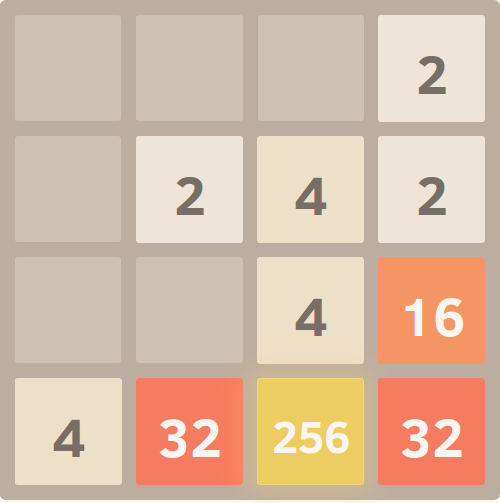
\includegraphics[width=5cm]{img/2048.png}
    \caption{How the screen representation of the \texttt{b} array (table \ref{array_b}) would look.}
\end{figure}

\newpage
\subsection{Gamepad input}
Upon starting the game program, the gamepad driver listening is initialized by the function \texttt{init\_gamepad}.

\noindent{
\begin{minipage}{\linewidth}
\begin{lstlisting}[language=C, label=init_gamepad, caption=Initializing the gamepad driver listening]
int init_gamepad()
{
    device = fopen("/dev/gamepad", "rb");
    if (!device) {
        printf("Unable to open driver device, maybe you didn't load the module?\n");
        return EXIT_FAILURE;
    }
    if (signal(SIGIO, &sigio_handler) == SIG_ERR) {
        printf("An error occurred while register a signal handler.\n");
        return EXIT_FAILURE;
    }
    if (fcntl(fileno(device), F_SETOWN, getpid()) == -1) {
        printf("Error setting pid as owner.\n");
        return EXIT_FAILURE;
    }
    long oflags = fcntl(fileno(device), F_GETFL);
    if (fcntl(fileno(device), F_SETFL, oflags | FASYNC) == -1) {
        printf("Error setting FASYNC flag.\n");
        return EXIT_FAILURE;
    }
    return EXIT_SUCCESS;
}
\end{lstlisting}
\end{minipage}
}

This sets up the program so that when the driver registers an interrupt, the function \texttt{sigio\_handler()} is called.

\noindent{
\begin{minipage}{\linewidth}
\begin{lstlisting}[language=C, label=sigio_handler, caption=Input handler function]
void sigio_handler(int signo)
{
    int input = map_input(fgetc(device));
    switch (input) {
        case 1:
            left();
            break;
        case 2:
            up();
            break;
        case 3:
            right();
            break;
        case 4:
            down();
            break;
        case 6:
            if (last_input == 6) {
                new_game();
            }
            break;
        case 8:
            if (last_input == 8) {
                running = false;
            }
            break;
    }
    last_input = input;
}

\end{lstlisting}
\end{minipage}
}

The gamepad driver gives a bit string that represents the state of each of the eight buttons.
For this game, we were not interested in any button press combinations, so we used the function we defined in exercise 2 to map the input to a number representing a single button pressed.

\noindent{
\begin{minipage}{\linewidth}
\begin{lstlisting}[language=C, label=map_input, caption=Input decoding function]
int map_input(int input)
{
    input = ~input;
    for ( int i = 0; i < 8; i++) {
        int match = input & (1 << i);
        if ( (1 << i) == match ) {
            return (i+1);
        }
    }
    return 0;
}
\end{lstlisting}
\end{minipage}
}

\newpage
\subsection{Using the development board LED display}
As advised in the compendium, we used memory mapping to manipulate the image to be displayed.

\noindent{
\begin{minipage}{\linewidth}
\begin{lstlisting}[language=C, label=map_input, caption=Input decoding function]
int init_framebuffer()
{
    fbfd = open("/dev/fb0", O_RDWR);
    if (fbfd == -1) {
        printf("Error: unable to open framebuffer device.\n");
        return EXIT_FAILURE;
    }

    // Get screen size info
    if (ioctl(fbfd, FBIOGET_VSCREENINFO, &vinfo) == -1) {
        printf("Error: unable to get screen info.\n");
        return EXIT_FAILURE;
    }

    screensize_pixels = vinfo.xres * vinfo.yres;
    screensize_bytes = screensize_pixels * vinfo.bits_per_pixel / 8;

    fbp = (uint16_t*)mmap(NULL, screensize_bytes, PROT_READ | PROT_WRITE, MAP_SHARED, fbfd, 0);
    if ((int)fbp == MAP_FAILED) {
        printf("Error: failed to memorymap framebuffer.\n");
        return EXIT_FAILURE;
    }

    return EXIT_SUCCESS;
}
\end{lstlisting}
\end{minipage}
}

This maps a region of memory, identified by the pointer \texttt{fbp}, to \texttt{/dev/fb0}, also known as the development board LED display.

\subsubsection{Using fonts}
